\begin{frame}
\frametitle{Avionics}
\begin{center}
Automatic Dependent Surveillance -- Broadcast
\par
ADS-B
\end{center}
\end{frame}

\begin{frame}
\frametitle{ADS-B}
\begin{center}
ADS-B is an electronic system aboard aircraft that broadcasts certain information about that aircraft, to other aircraft, air traffic control on the ground and anyone else who chooses to receive the signal.
\end{center}
\end{frame}

\begin{frame}
\frametitle{ADS-B}
\begin{block}{ADS-B}
\begin{itemize}
\item<1-> The ICAO identifier for the airframe.
\item<2-> The flight identifier e.g. aircraft callsign.
\item<3-> Aircraft position.
\item<4-> The integrity of the position report e.g. GPS accuracy.
\item<5-> Altitude as a function of barometric pressure.
\item<6-> Altitude as a function of GPS.
\item<7-> Rate of climb/descent.
\item<8-> Aircraft ground track.
\item<9-> Aircraft ground speed.
\item<10-> Any emergency indicators.
\end{itemize}
\end{block}
\end{frame}

\begin{frame}
\frametitle{ADS-B}
\begin{block}{ADS-B}
\begin{itemize}
\item<1-> ADS-B has a revision history in \emph{modes}.
\item<2-> Mode-S is broadcast on 1090MHz\footnote{also 978MHz in some countries e.g. USA}.
\item<3-> Mode-S is most recent and can be received without transmitting\footnote{unlike Mode-C}.
\item<4-> All IFR aircraft must be Mode-S ADS-B equipped by 2017.
\end{itemize}
\end{block}
\end{frame}

\begin{frame}
\frametitle{ADS-B}
\begin{block}{ADS-B receive}
\begin{itemize}
\item<1-> We can receive Mode-S ADS-B signals with a SDR.
\item<2-> Raspberry-pi, DVB Tuner, 1090MHz antenna.
\end{itemize}
\end{block}
\end{frame}

\begin{frame}
\frametitle{ADS-B}
\begin{block}{You are no doubt wondering}
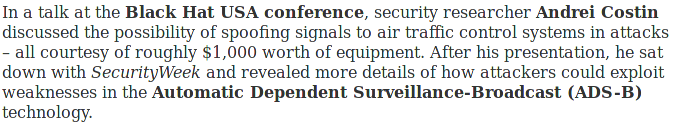
\includegraphics[height=0.18\textheight]{image/adsb-security.png}
\end{block}
Yes the absence of security in ADS-B has been demonstrated.
\end{frame}

\begin{frame}
\frametitle{Portable ADS-B receiver hardware}
\begin{block}{Portable ADS-B receiver hardware}
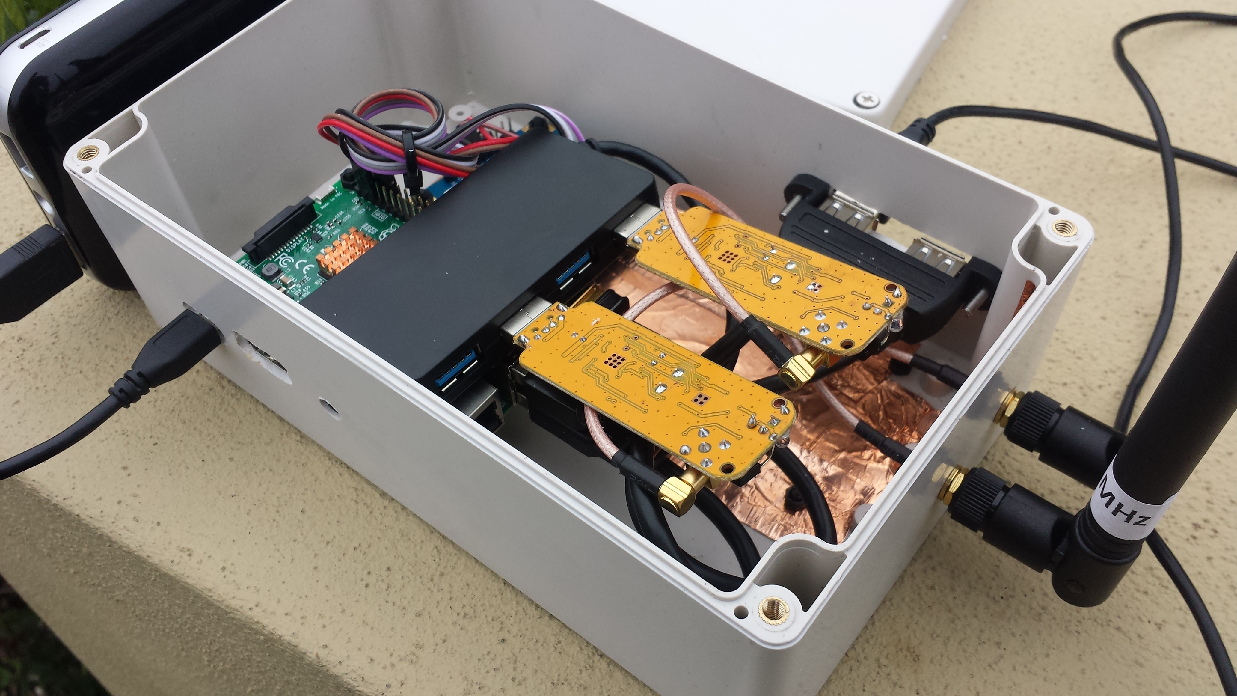
\includegraphics[height=0.5\textheight]{image/adsb-hardware.png}
\end{block}
\end{frame}

\begin{frame}
\frametitle{Portable ADS-B receiver hardware}
\begin{block}{RTL2832U Digital DVB-T (x2)}
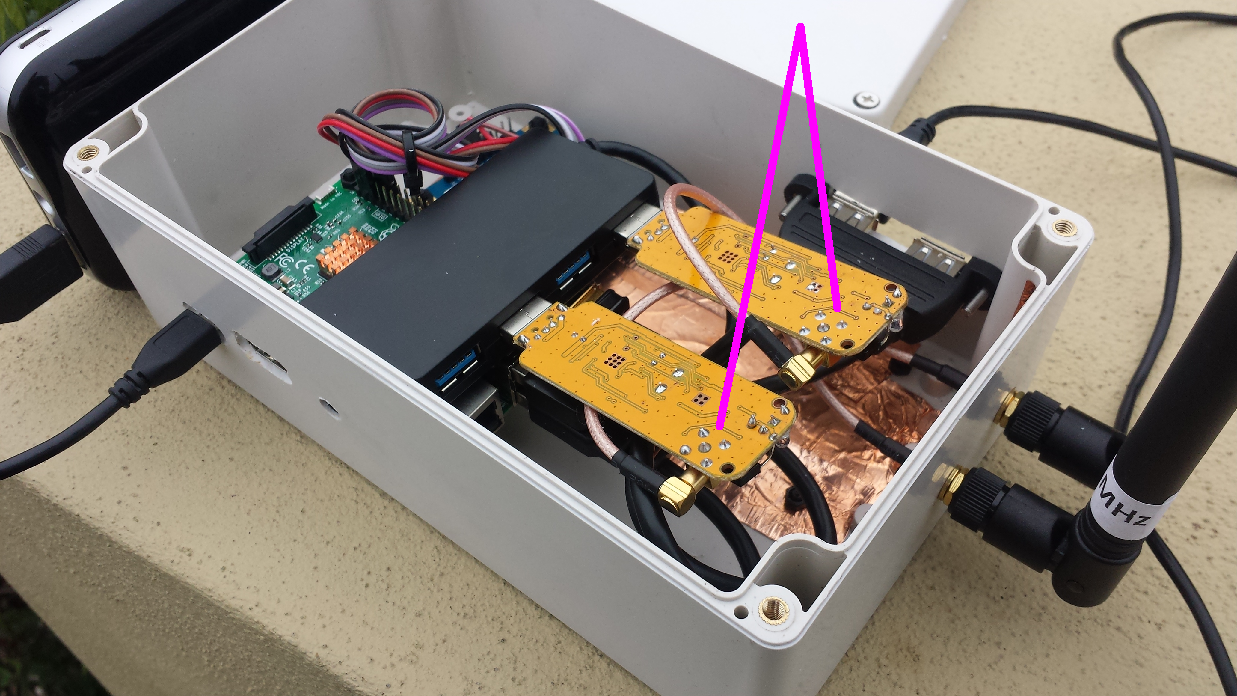
\includegraphics[height=0.5\textheight]{image/adsb-hardware-dvb.png}
\begin{itemize}
\item RTL2832U Digital DVB-T to receive 1090MHz.
\item 2x for either adding 978MHz or redundant 1090MHz.
\end{itemize}
\end{block}
\end{frame}

\begin{frame}
\frametitle{Portable ADS-B receiver hardware}
\begin{block}{Dual 1090MHz Antennae}
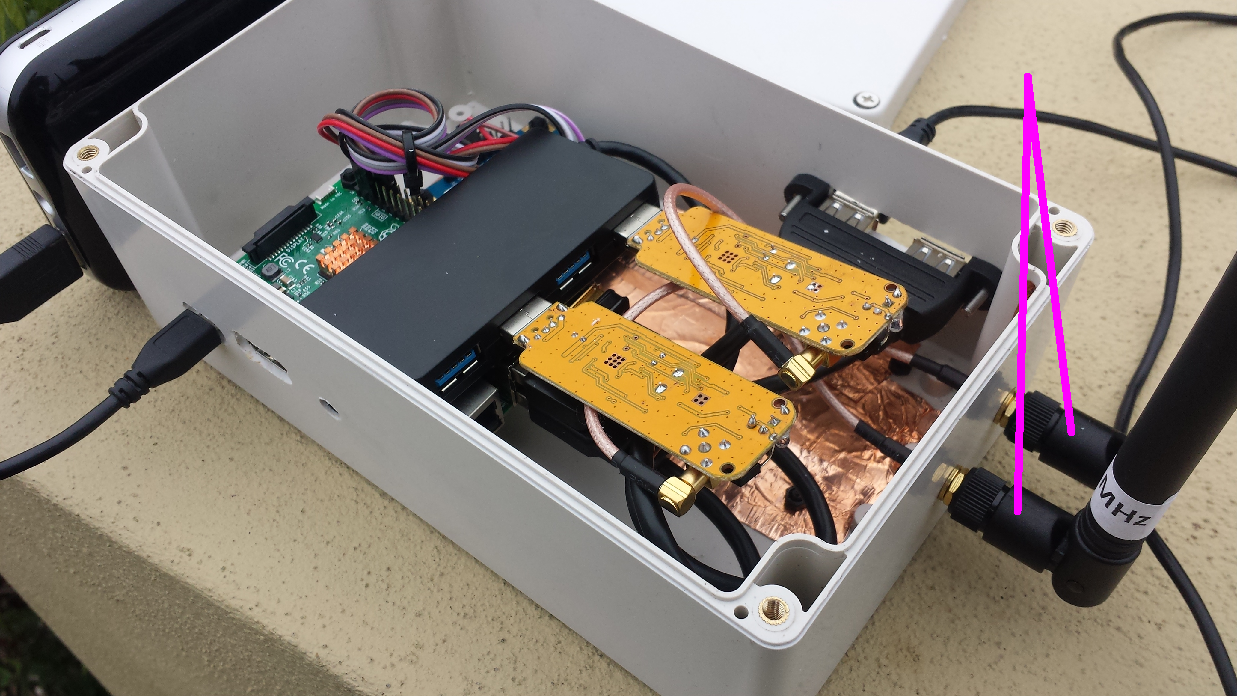
\includegraphics[height=0.5\textheight]{image/adsb-hardware-antennae.png}
\begin{itemize}
\item Copper ground plane can be seen.
\end{itemize}
\end{block}
\end{frame}

\begin{frame}
\frametitle{Portable ADS-B receiver hardware}
\begin{block}{VK-162 GPS}
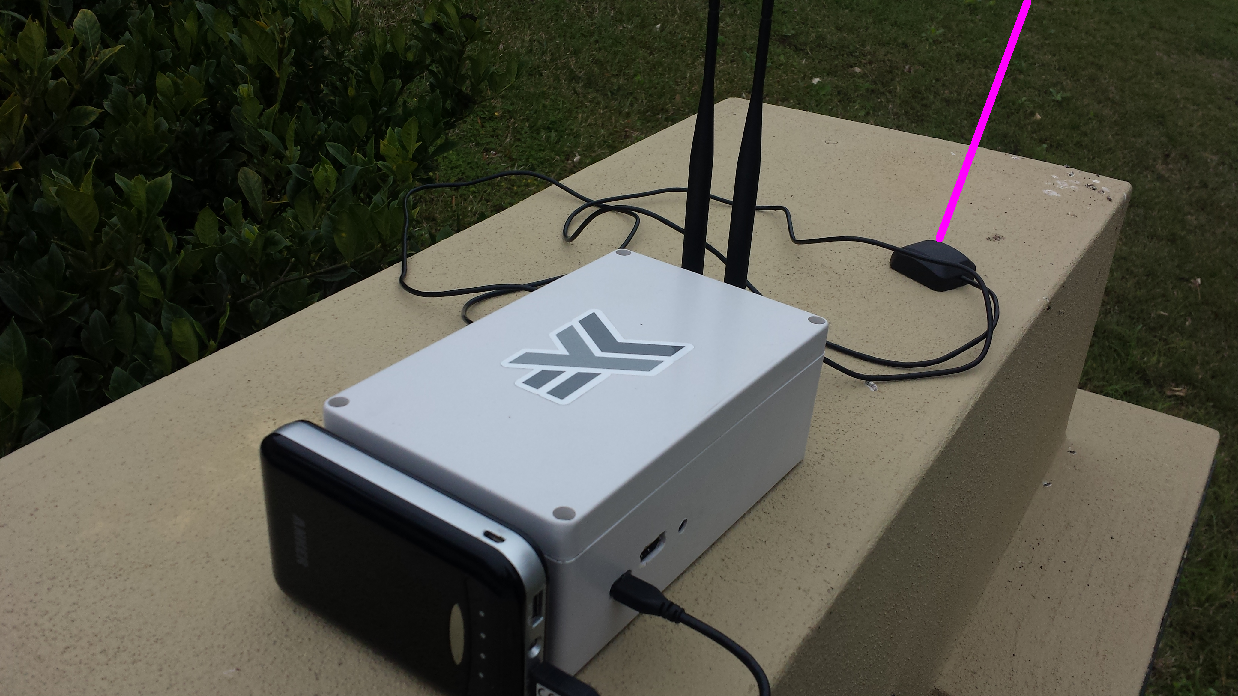
\includegraphics[height=0.5\textheight]{image/adsb-hardware-vk162.png}
\begin{itemize}
\item External GPS antenna with magnetic mount.
\item Provides track.
\item Provides ground speed.
\end{itemize}
\end{block}
\end{frame}

\begin{frame}
\frametitle{Portable ADS-B receiver hardware}
\begin{block}{RY835AI}
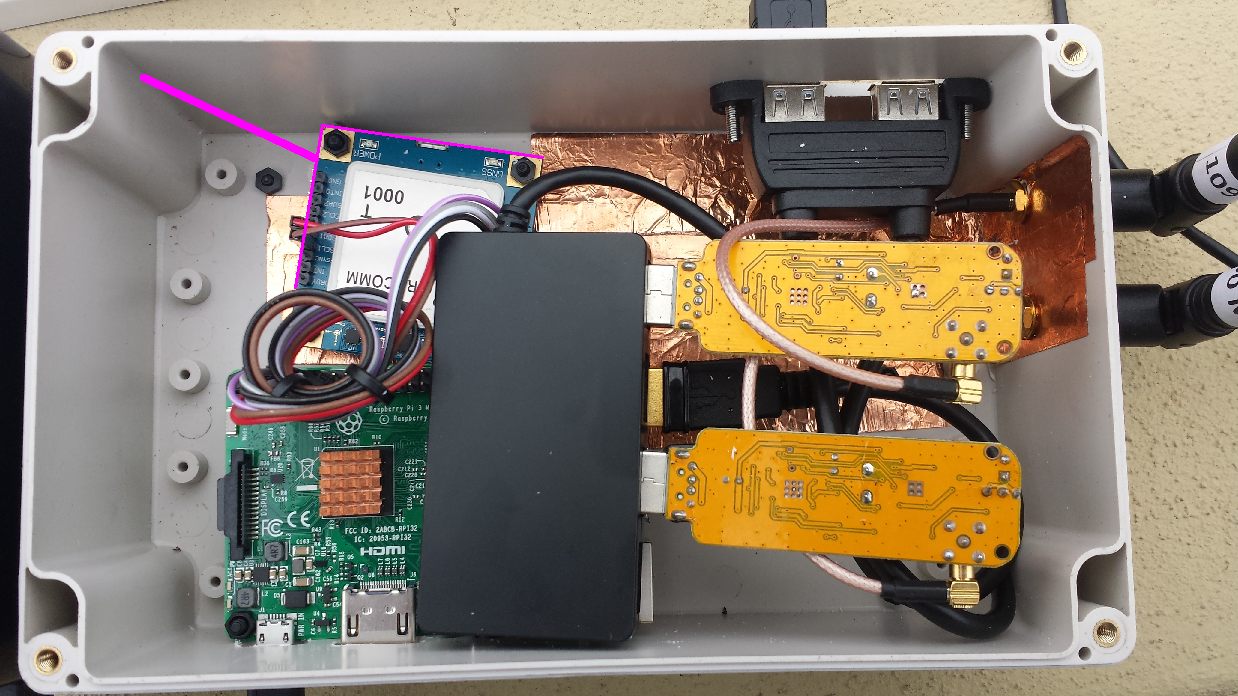
\includegraphics[height=0.5\textheight]{image/adsb-hardware-ry835ai.png}
\tiny
\begin{itemize}
\item Gyrometer providing roll, pitch and yaw.
\item Magnetometer provides magnetic heading \& lateral orientation.
\item Barometer provides air pressure (altitude).
\item Thermometer provides outside air temperature.
\end{itemize}
\end{block}
\end{frame}

\begin{frame}
\frametitle{Portable ADS-B receiver hardware}
\begin{block}{Today's challenge}
To physically place this device such that:
\begin{itemize}
\item<1-> It can receive ADS-B from Melbourne air traffic.
\item<1-> It can connect to the WLAN in my pocket.
\item<2-> Nobody finds it, or we really will be evacuated.
\end{itemize}
\end{block}
\end{frame}

\begin{frame}
\frametitle{Portable ADS-B receiver software}
\begin{block}{Stratux GPS/AHRS web}
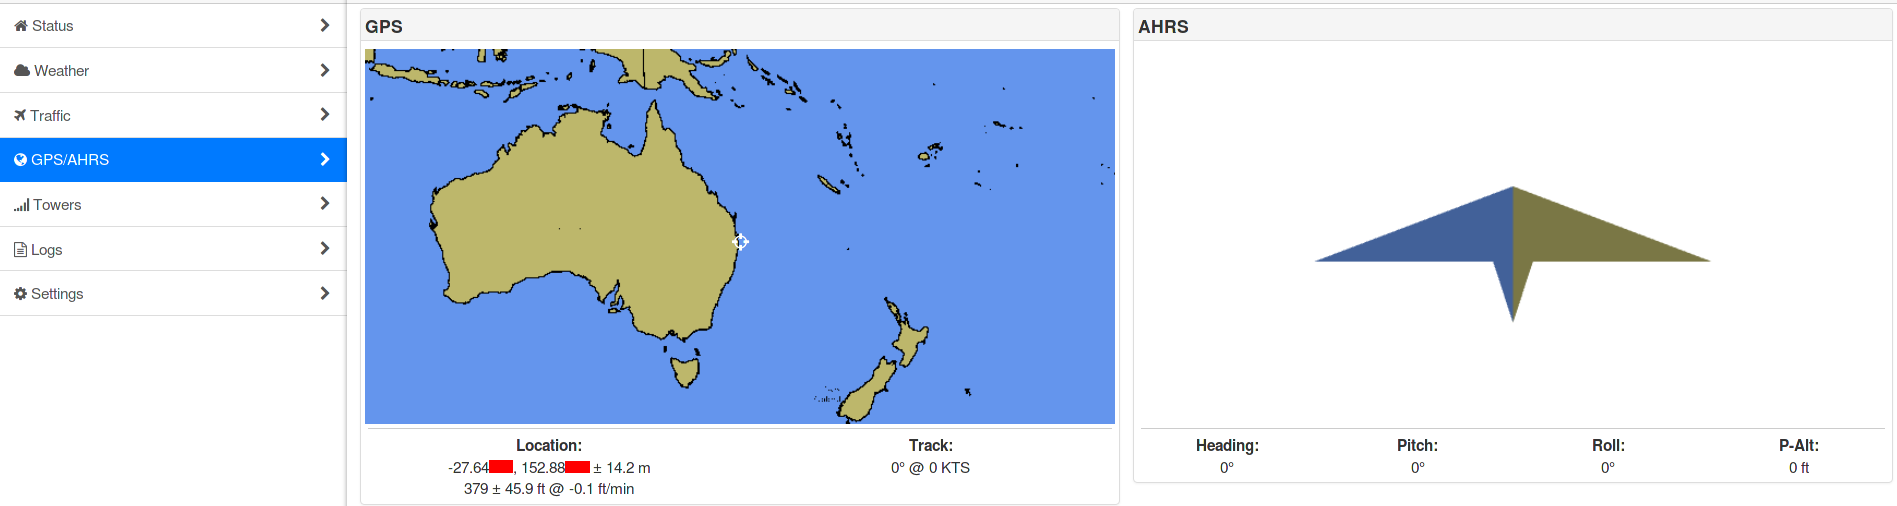
\includegraphics[height=0.32\textheight]{image/stratux-gps-ahrs-web.png}
\end{block}
\end{frame}

\begin{frame}
\frametitle{Portable ADS-B receiver software}
\begin{block}{Stratux Traffic web}
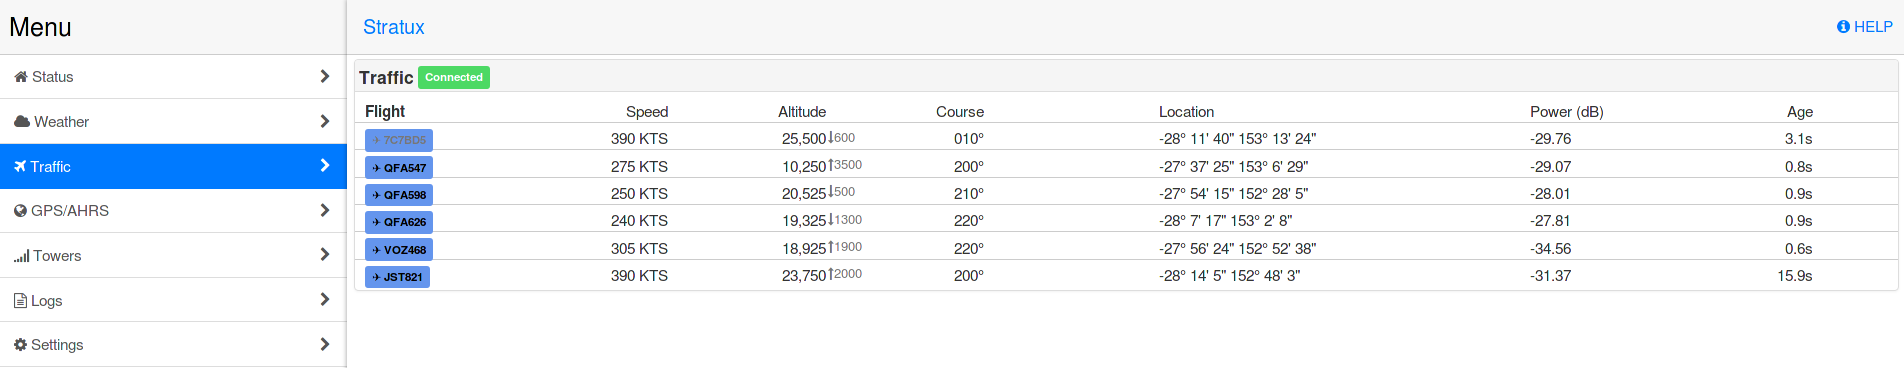
\includegraphics[height=0.23\textheight]{image/stratux-traffic-web.png}
\end{block}
\end{frame}

\begin{frame}
\frametitle{Portable ADS-B receiver software}
\begin{block}{Traffic record data type}
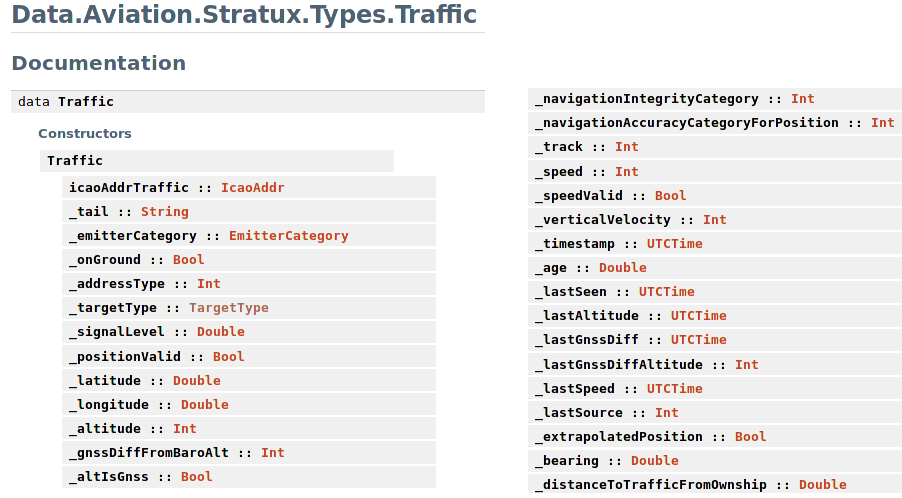
\includegraphics[height=0.6\textheight]{image/stratux-traffic-record.png}
\end{block}
\end{frame}

\begin{frame}
\frametitle{Portable ADS-B receiver software}
\begin{block}{Situation record data type}
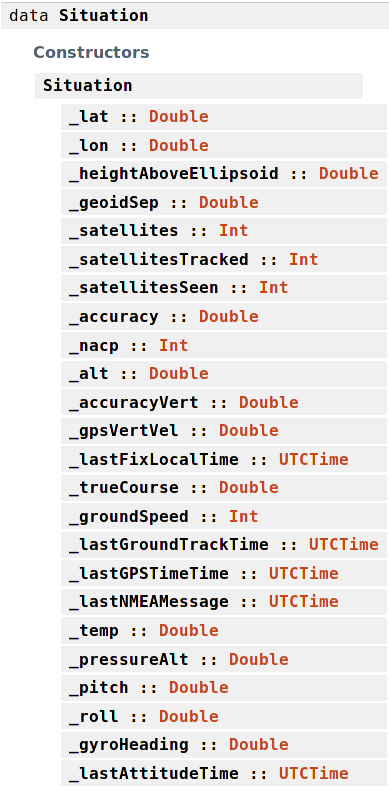
\includegraphics[height=0.6\textheight]{image/stratux-situation-record.png}
\end{block}
\end{frame}

\begin{frame}
\frametitle{Portable ADS-B receiver software}
\begin{center}
Let's code!
\end{center}
\end{frame}
